\documentclass{standalone}
\usepackage{tikz}
\usepackage{pgfplots}
\pgfplotsset{compat=newest}
\usepackage{amsmath}
\usepackage[american]{circuitikz}
\usepackage{cmbright}

\definecolor{myred}{RGB}{170,0,0}
\definecolor{myblue}{RGB}{0,0,220}
\definecolor{mygreen}{RGB}{0,150,0}
\definecolor{myorange}{RGB}{255,127,0}
\definecolor{mybrown}{RGB}{150,75,0}

\ctikzset{bipoles/resistor/height=0.2}
\ctikzset{bipoles/resistor/width=0.5}

\begin{document}
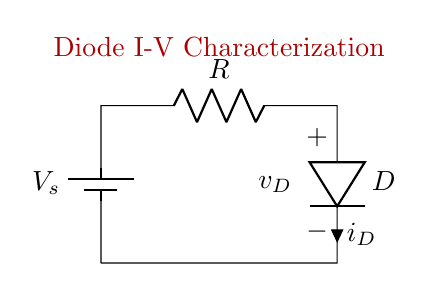
\begin{tikzpicture}
    % Diode circuit
    \begin{scope}
        \node[anchor=center, color=myred, align=center] at (1.5, 2.75) {Diode I-V Characterization};
        \draw (0,0) 
            to[battery1, l={$V_s$}, invert] ++(0, 2)
            to[R, l={$R$}] ++(3, 0)
            to[D, l=$D$, i^>=$i_D$, v_={$v_D$}] ++(0, -2) 
            to[short] ++(-3, 0);
    \end{scope}
\end{tikzpicture}
\end{document}